\documentclass[10pt]{beamer}

\usetheme[progressbar=frametitle]{metropolis}

\include{preamble}

\usepackage{booktabs}
\usepackage[scale=2]{ccicons}

%\usepackage{pgfplots}
%\usepgfplotslibrary{dateplot}

\usepackage{xspace}
\newcommand{\themename}{\textbf{\textsc{metropolis}}\xspace}

\title{Algorithms for Scheduling and Routing Problems}
\subtitle{Ph.D. Thesis Seminar Presentation}
\date{\today}
\author{Kamyar Khodamoradi}
\institute{Simon Fraser University \\ School of Computing Science}
\titlegraphic{\hfill\includegraphics[height=0.75cm]{logo_sfu}}

\begin{document}

\maketitle

\begin{frame}{Table of contents}
  \setbeamertemplate{section in toc}[sections numbered]
  \tableofcontents[hideallsubsections]
\end{frame}

%%%%%%%%%%%%%%%%%%%%%%%%%%%%%%%%%%%%%%%%%%%%%%%%%%%%%%%%%%%%%%%%%%%%%%%%%%%%%%%%%%%%%%%%%%%%%%%%%%%%%%%%%%%%%%%%%%%%%%%%%%%%%%%
\section{Indivisible Resource Allocation}

\begin{frame}{Introduction} 
\begin{itemize}
	\item<1-> \alert{Resource Allocation}: allocation of scarce resources to customers while satisfying some given constraints
    \item<2-> First publication were in the 1950's in industrial engineering and operations research
    \item<3-> Various applications in computer science, operations research, etc.:
    \begin{itemize}
		\item<4-> Production planning
		\item<5-> On-line auctions
    	\item<6-> Operating systems design 
        \item<7-> Computer networks 
        \item<8-> Wireless communications
        \item<9-> $\ldots$
	\end{itemize}	
	\item <10-> Both theoretically and practically important
\end{itemize}
\end{frame}

\begin{frame}{Two Types of Resource Allocation}
\begin{itemize}
	\item<1-> Based on the type of resource, two sub-categories emerge:
	\begin{enumerate}
		\item<2-> Divisible 
		\item<3-> Indivisible
	\end{enumerate}
	\item<4-> The Divisible case is also known as the ``cake-cutting'' problem
	\item<5-> The question: \emph{fair division} of divisible resources
	\item<6-> Mostly studied in  economics, game theory, and sociology 
\end{itemize}
\end{frame}

\begin{frame}{Indivisible Resource Allocation (IRA)}
\begin{itemize}
	\item<1-> A fundamental problem in combinatorial optimization and operation research	
	\item<2-> Four main components:
	\begin{enumerate}
		\item<3-> a set $\cR$ of $n$ unsplittable resources
		\item<4-> a set $\cP$ of $m$ players
		\item<5-> a \alert{utility} function $f_{i}: \, 2^{\cR} \rightarrow \R$ for each $i \in \cP$ (representing the item bundles values for player $i$)
		\item<6-> an objective function on \alert{allocations}
	\end{enumerate}
\end{itemize}
\begin{definition}[Allocation]<7->
An allocation $\cA$ for an instance of a \textsc{IRA} problem is a partition of $\cR$ into $m$ sets $\cA_{1}, \cA_{2}, \ldots, \cA_{m}$.
\end{definition}
\end{frame}

\begin{frame}{Example 1. Scheduling I}
\begin{itemize}
	\item<1-> Scheduling is one of the classic problems in combinatorial optimization
	\item<3-> Scheduling and resource allocation have many similarities
	\item<4-> Scheduling problems can usually be cast as resource allocation problems and vice versa    
	\begin{example}
	    Given:
        \begin{itemize}
            \item<6-> A set of jobs
            \item<7-> A set of processors (machines)
            \item<8-> Processing times
            \item<9-> An objective functions: minimize the makespan, sum of processing times, $\ldots$
        \end{itemize}
    \end{example}
\end{itemize}
\end{frame}

\begin{frame}{Example 1. Scheduling II}
\begin{figure}
    \begin{center}
        \includegraphics[width=9cm]{Scheduling.eps}
    \end{center}
\end{figure}
\end{frame}


\begin{frame}{Example 2. Vehicle Routing}
\begin{itemize}
    \item<1-> Vehicle Routing problem (VRP) is a major problem in the logistics and delivery services
    \item<2-> VPR can also be viewed as an IRA problem.
    \begin{example}
        Given: 
        \begin{itemize}
            \item<3-> A fleet of vehicles
            \item<4-> A set of clients spread over an area 
            \item<5-> Travel costs
            \item<6-> An objective function: minimize the sum of the travel costs
            \item<7-> Extra constraints: time windows, skill requirements, $\ldots$
        \end{itemize}        
    \end{example}
\end{itemize}
    
\end{frame}

%%%%%%%%%%%%%%%%%%%%%%%%%%%%%%%%%%%%%%%%%%%%%%%%%%%%%%%%%%%%%%%%%%%%%%%%%%%%%%%%%%%%%%%%%%%%%%%%%%%%%%%%%%%%%%%%%%%%%%%%%%%%%%%
\section{Skill Vehicle Routing Problem}

\begin{frame}{Introduction I}
\begin{example}
    \begin{center}
            \includegraphics[width=8cm]{VRPSS01.pdf} 
    \end{center}
\end{example}
\end{frame}

\begin{frame}{Introduction II}
\begin{example}
    \begin{center}
            \includegraphics[width=8cm]{VRPSS03.pdf} 
    \end{center}
\end{example}
\end{frame}

\begin{frame}{Introduction III}
\begin{itemize}
    \item<1-> A set of \alert{customers} $S$
    \item<2-> A skill requirement $q_j$ for each customer $j \in S$
    \item<3-> A fleet of vehicles (\alert{drivers}) $D$
    \item<4-> A set of skills $K_i$ for each driver $i \in D$
    \item<5-> Metric graph $G = (S, \, E)$ (on a Euclidean plane) 
    \item<6-> A special node \emph{depot}, $r \in S$
    \item<7-> A cost function $c:E \rightarrow \bR^+$ for every pair of nodes
\end{itemize}
\end{frame}

\begin{frame}{Introduction IV}
\begin{itemize}
    \item<1-> The goal is to find routes that start and end at $r$ and assign them to drivers such that
    \begin{itemize}
        \item<2-> The union of all the tours cover $S$
        \item<3-> The drivers can served the customers assigned to them
        \item<4-> The total travel distance is minimized
    \end{itemize}
    \item<5-> We seek optimal or \emph{provably near-optimal } solutions because:
        \begin{itemize}
            \item<6-> Vehicle routing problems are becoming more and more recurrent (if the problem size allows optimal solution)
            \item<7-> Optimal solutions can serve as a benchmark for heuristic solutions (for prohibitively large instances)
        \end{itemize}
\end{itemize}
\end{frame}


\begin{frame}{Background}
\begin{itemize}
    \item<1-> Linear Programming (LP) is the model of choice for obtaining exact solutions
    \item<2-> Many researchers have used a \alert{Delayed Column Generation} technique (Column Generation) in the context of VRP with \emph{time windows}
    \item<3-> Column generation works very well for LP formulations with large number of variables
    \item<4-> See \cite{DDS05} for an extensive list of work
\end{itemize}
\end{frame}

\begin{frame}{Column Generation I}
\begin{itemize}
    \item<1-> An ILP formulation with small integrality gap:
    \item<2->[ ] \begin{align}
        \text {min } \label{cg_obj}	 \sum_{ i, 	T \in \cT(i) } z_{i, T} & \cdot C(T) &    &  \\
        \text{subject to }             & & \nonumber  \\
        \label{const:cg1}       \sum_{ T \in \cT(i) } z_{ i, T } & = 1  &   \forall i \in D \\
        \label{const:cg2}       \sum_{ i, T \in \cT(i): T \ni j } z_{ i, T } & \geq 1   &   \forall j \in S \\
        \label{consT:cg3}       z_{ i, T } & \in \{0,\, 1\}    & \forall \, i \in D, \, \forall \, T \in \cT(i) 
    \end{align}
    \item<3-> An indicating variable $z_{i, T}$ for every possible \alert{tour} $T$ and every driver $i$
    \item<4-> $\cT(i)$: set of tours serviceable by driver $i$
\end{itemize}
\end{frame}

\begin{frame}{Column Generation II}
\begin{itemize}
    \item<1-> Exponential number of variables $z_{i, T}$
    \item<2-> Column generation: do not introduce them all at once
    \item<3-> We use column generation in an iterative frame work: \alert{Branch-and-Price}
    \begin{itemize}
        \item<4-> A \alert{Branch-and-Cut} on the dual formulation
        \item<5-> Uses the column generation technique in a branch-and-bound algorithm
    \end{itemize}
\end{itemize}
\end{frame}

\begin{frame}{Branch-and-Price I}
\begin{center}
        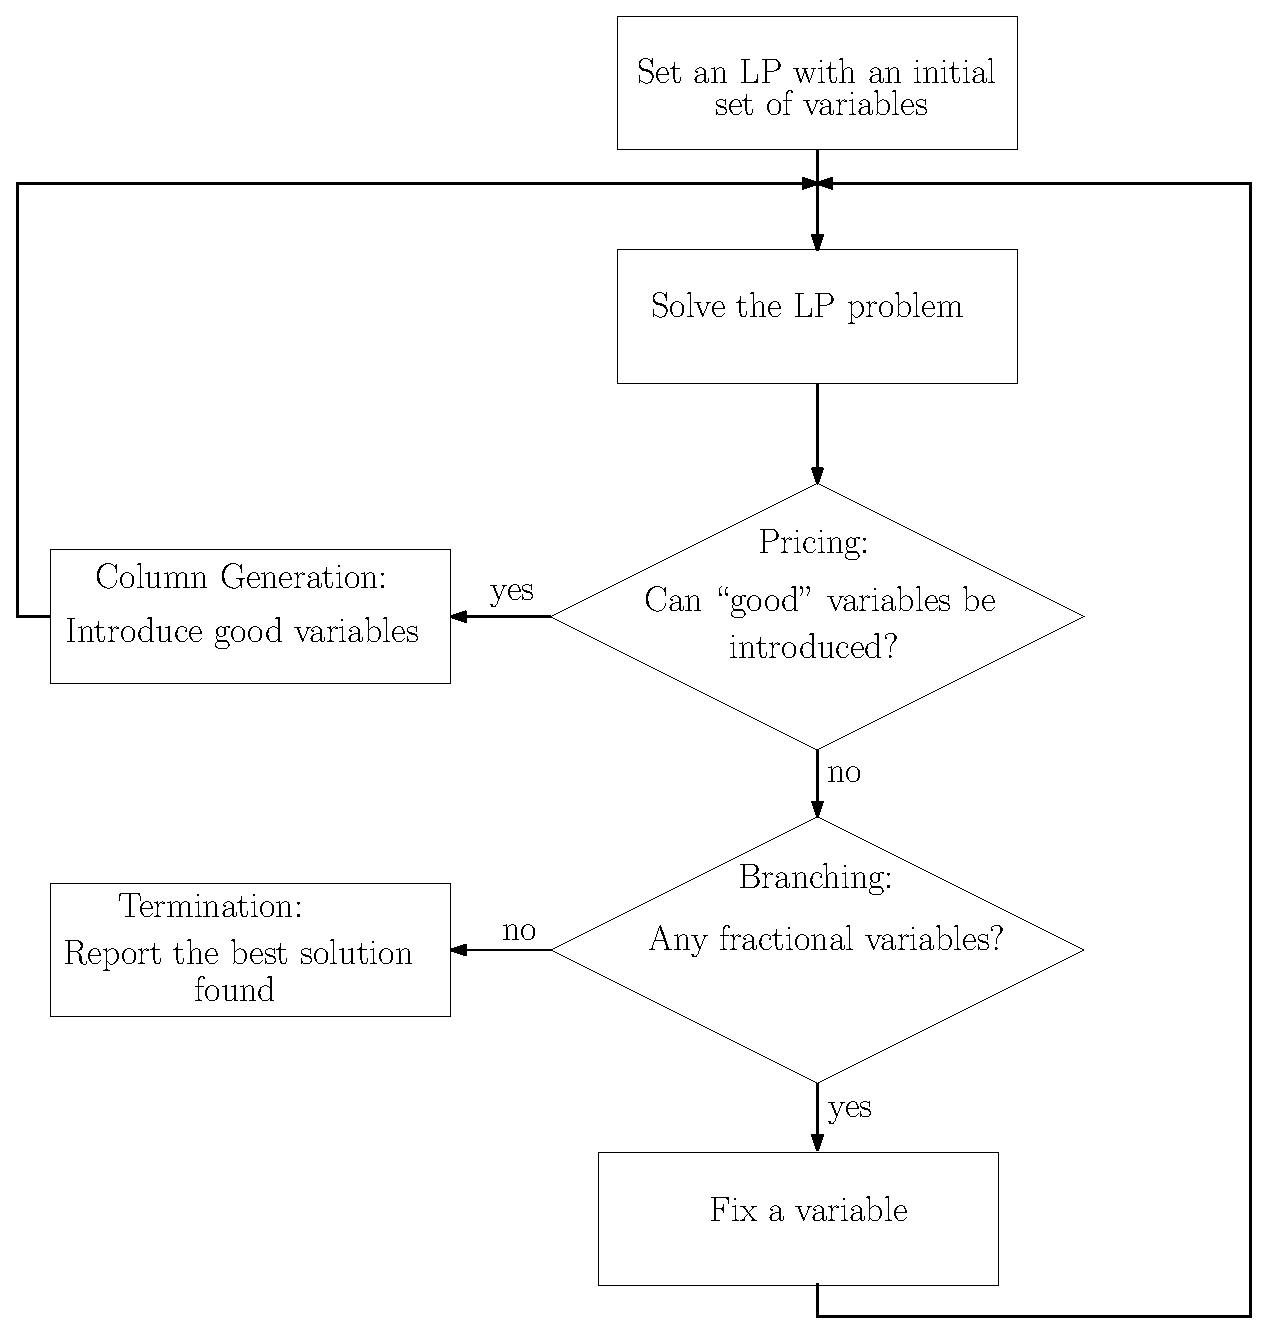
\includegraphics[width=7cm]{Branch_and_Price.eps} 
\end{center}
\end{frame}

\begin{frame}{Branch-and-Price II}
\begin{itemize}
    \item<1-> Pricing: finding ``good'' variables to add to the model
    \begin{itemize}
        \item<2-> A \alert{reduced cost} column
        \item<3-> Finding such a column is a problem of its own (\alert{subproblem})
        \item<4-> For SVRP, the subproblem is the \alert{Prize-Collecting TSP} (PCTSP)
    \end{itemize}
    \item<5-> Branching: use heuristics to decide which variable to \emph{fix}
    \item<6-> Bounding: if the current LP has an objective value worse than the best known so far, abandon this LP and go the next (not shown in the flowchart)
    \item<7-> Termination: when no more reduced cost columns or fractional variables, return the best solution (the \alert{incumbent})
\end{itemize}
\end{frame}


%%%%%%%%%%%%%%%%%%%%%%%%%%%%%%%%%%%%%%%%%%%%%%%%%%%%%%%%%%%%%%%%%%%%%%%%%%%%%%%%%%%%%%%%%%%%%%%%%%%%%%%%%%%%%%%%%%%%%%%%%%%%%%%
\section{Prize-Collecting Traveling Salesman Problem}


\begin{frame}[fragile]{Introduction}

\begin{itemize}
\item<1-> A variant of the Traveling Salesman Problem (TSP)
\item<2-> Metric graph $G = (S, \, E)$ (on a Euclidean plane) 
\item<3-> A special node ``depot'', $r \in S$
\item<4-> A cost function $c:E \rightarrow \bR^+$ for every pair of nodes
\item<5-> A prize function $\beta:S \rightarrow \bR^+$ for every node
\item<6-> \alert{Objective:} Find a tour covering the depot and \alert{some} other nodes, maximizing the sum of prizes minus the sum of costs

\end{itemize}
\end{frame}

\begin{frame}[fragile]{An Example I}

\begin{itemize}
\item An instance of the Prize Collecting TSP:
\begin{figure}
	\centering
	\begin{tikzpicture}
        
        \draw (0, 0) node[circle, inner sep=1pt, fill=black, label={below:{$depot$}}] (D) {}; 
        \draw (1, 1) node[circle, inner sep=1pt, fill=black] (A) {}; 
        \draw (3, 2) node[circle, inner sep=1pt, fill=black] (B) {}; 
        \draw (-3, 3) node[circle, inner sep=1pt, fill=black] (C) {}; 
        \draw (-1, 4) node[circle, inner sep=1pt, fill=black] (E) {}; 
        \draw (0, 3) node[circle, inner sep=1pt, fill=black] (F) {}; 
        \draw (2, 3) node[circle, inner sep=1pt, fill=black] (G) {}; 
         \draw (-3, 1) node[circle, inner sep=1pt, fill=black, label={below:{$v$}}] (v) {}; 
        \draw (-2, 2) node[circle, inner sep=1pt, fill=black, label={below:{$u$}}] (u) {};         
        \node at (-2.5, 1.5) (m) {};
        \node at (-4, 1.5) (n) {$c_{uv}$};
        
        \draw [->, color = red] (m) to [bend right = 45] (n);
        \draw [fill = blue, dashed, thick] (u) to (v);

    	\node[above = 0.2cm] at (-2, 2) {$\beta_u$};
	\end{tikzpicture}
    \caption{Prize Collecting TSP}
    \label{fig:intersect_intervals}
\end{figure}
\end{itemize}
\end{frame}

\begin{frame}[fragile]{An Example II}

\begin{itemize}
\item Solution value $ = (6 + 2 + 7 + 10 + 4) - (3.2  + 1.4 + 2.2 + 3.2 + 2.2 + 1.4) = $ \alert{15.4}
\begin{figure}
	\centering
	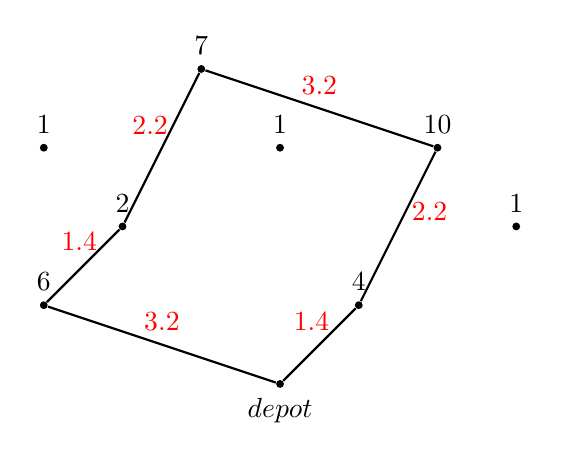
\begin{tikzpicture}
        
        \draw (0, 0) node[circle, inner sep=1pt, fill=black, label={below:{$depot$}}] (D) {}; 
        \draw (1, 1) node[circle, inner sep=1pt, fill=black, label = {above:{4}}] (A) {}; 
        \draw (3, 2) node[circle, inner sep=1pt, fill=black, label = {above:{1}}] (B) {}; 
        \draw (-3, 3) node[circle, inner sep=1pt, fill=black, label = {above:{1}}] (C) {}; 
        \draw (-1, 4) node[circle, inner sep=1pt, fill=black, label = {above:{7}}] (E) {}; 
        \draw (0, 3) node[circle, inner sep=1pt, fill=black, label = {above:{1}}] (F) {}; 
        \draw (2, 3) node[circle, inner sep=1pt, fill=black, label = {above:{10}}] (G) {}; 
         \draw (-3, 1) node[circle, inner sep=1pt, fill=black, label = {above:{$6$}}] (v) {}; 
        \draw (-2, 2) node[circle, inner sep=1pt, fill=black, label = {above:{$2$}}] (u) {};                 
        \draw [fill = blue, thick] (D) to (v) to (u) to (E) to (G) to (A) to (D);
        \node [above = 0.05cm, color = red] at (-1.5, 0.5) {3.2};
        \node [above = 0.07cm, color = red] at (-2.55, 1.5) {1.4};
        \node [above = 0.05cm, color = red] at (-1.65, 3) {2.2};
        \node [above = 0.05cm, color = red] at (0.5, 3.5) {3.2};
        \node [above = 0.05cm, color = red] at (1.9, 1.9) {2.2};
        \node [above = 0.05cm, color = red] at (0.4, 0.5) {1.4};
        
	\end{tikzpicture}
    \caption{A feasible solution to PCTSP}
    \label{fig:intersect_intervals}
\end{figure}
\end{itemize}
\end{frame}

\begin{frame}[fragile]{Other Names: Penalty TSP}
\begin{itemize}
\item<1-> Alternatively, every node $v$ may have a penalty $\beta_v$. 
\item<2-> Objective: cover the depot and some other nodes minimizing the cost plus penalties for the uncovered nodes
\item<3-> Other names: Penalty Traveling Salesman Problem (PTSP)
\item<4-> Complexity: \NPH (optimization version)
\item<5-> Arises as the subproblem in column generation approaches to various vehicle routing problems
	\begin{itemize}
	\item<6-> e.g., the ``Skill Vehicle Routing Problem'' 	\cite{Cappanera2011}
	\item<7-> One needs to solve PCTSP to get reduced cost columns as well as \emph{upper bounds} on the objective value for the SVRP
    \end{itemize}
\end{itemize}
\end{frame}

\begin{frame}[fragile]{Background}
\begin{itemize}
    \item<1-> Introduced by Egon Balas \cite{Balas89}
    \item<2-> More general version:
	\begin{alertblock}{Prize Collecting TSP (PCTSP)}
		A complete graph with the cost and prize functions is given. Cover the depot and some other nodes, maximize the sum of prizes minus the sum of costs, Furthermore, guarantee the total sum of prizes is at least a \alert{prescribed} amount.
	\end{alertblock}
	\item<3-> Gendreau et al. \cite{GLS98} and Fischetti et al. \cite{FST97} have provided Branch-and-Cut algorithms for variants of the problem
    \item<4-> Some metaheuristics for the PCTSP are due to Chaves and Lorena \cite{Chaves08}
\end{itemize}
\end{frame}

\begin{frame}{Exact Solutions: A Branch-and-Cut Algorithm I}
\begin{itemize}
    \item<1-> Based on an ILP formulation:
    \item<2-> [ ] \begin{align} 
    \text {max } \label{pctsp_obj}     & \sum_{j\in S} \beta_j y_j  - \sum_{e\in E} c_e x_e &
    \\
    \text{subject to } \nonumber    &  & \\
    \label{const:pctsp1}               & \sum_{e \in \delta(i)} x_e = 2 y_{i}  & \forall i \in S \\
    \label{const:pctsp2}               & \sum_{e \in E(V) } x_e \leq \sum_{i \in V \backslash\{ k \}} y_{i} & \forall k \in V, V\subseteq S' \\
    \label{const:pctsp3}               & y_r = 1 \\
    \label{const:pctsp4}               & x_e \in \{0, \, 1\}, \, y_j \in \{0, \, 1\}  & \forall e \in E, \forall j \in S 
    \end{align}
    \item<3-> \constref{pctsp2} are referred to as the \alert{Generalized Subtour Elimination Constraints} (GSECs) 
\end{itemize}
\end{frame}

\begin{frame}{Exact Solutions: A Branch-and-Cut Algorithm II}
\begin{center}
        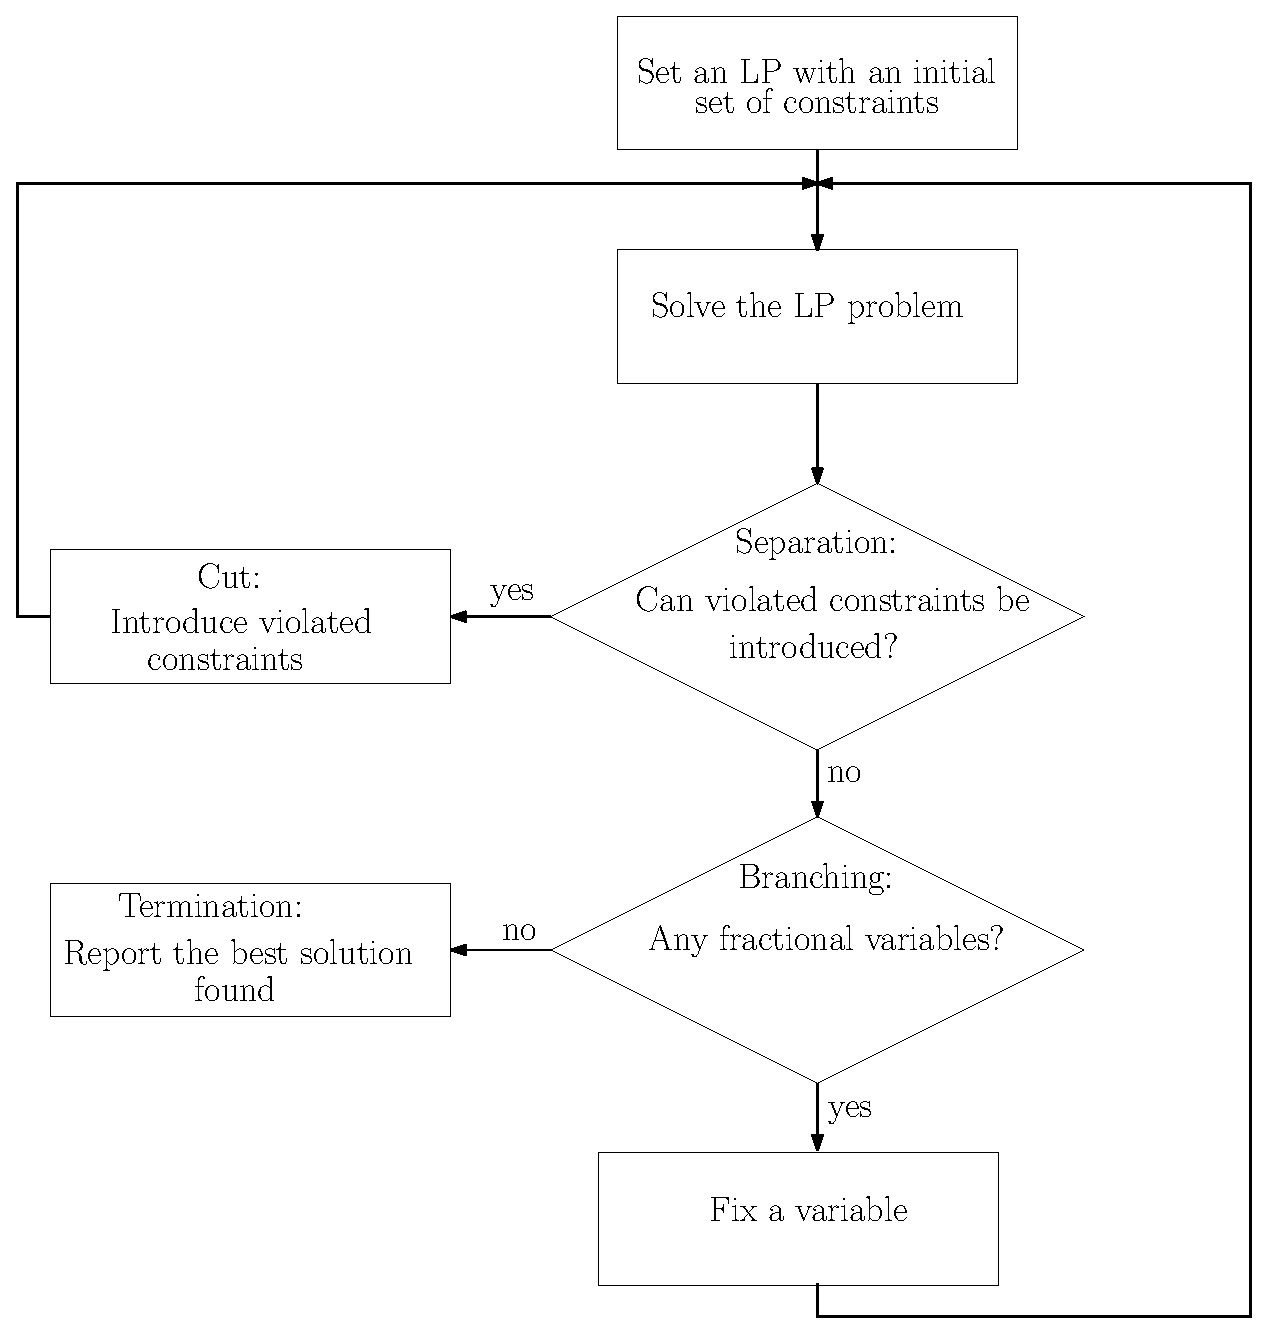
\includegraphics[width=7cm]{Branch_and_Cut.eps} 
\end{center}
\end{frame}

\begin{frame}[fragile]{More Background}
\begin{itemize}
    \item<3-> Balas studied cuts for the PCTSP problem
    \item<4-> Idea: Find equivalent or similar cuts for PCTSP as those of TSP
    \item<1-> Balas derives equivalent of Subtour Elimination Constraints (SEC) for PCTSP is 1989 \cite{Balas89}
    \item<2-> \alert{Generalized Subtour Elimination Constraints (GSEC)} introduced by Goemans in 1994 \cite{Goemans94} for Prize Collecting Steiner Tree problem
    \item<3-> For PCTSP, Balas finds the cuts corresponding to \alert{Primitive Comb Inequalities} (known for TSP) in 1995 \cite{Balas95}
\end{itemize}
\end{frame}


\begin{frame}{Our Contribution}
\begin{itemize}
    \item<1-> We developed a complete branch-and-cut algorithm:
    \begin{itemize}
        \item<2-> Fast separation heuristics that can detect two types of violated cuts:
        \begin{itemize}
            \item<3-> GSECs
            \item<4-> Primitive Comb Inequalities
        \end{itemize}
        \item<5-> Local search heuristics for improving the lower bound
        \item<6-> Branching heuristics for finding a good candidate variable to fix
    \end{itemize}
\end{itemize}
\end{frame}



\begin{frame}[fragile]{Background - Separation}
\begin{itemize}
\item<1-> Problem: exponential number of cuts
\item<2-> GSECs and Primitive Comb Inequalities need to be introduced gradually (through iterations)
\item<3-> \alert{Separation:} finding violated cuts in each iteration
\item<4-> Separation heuristics have been studied for variations of PCTSP
\begin{itemize}
\item<5-> e.g., for Quota Prize Collecting TSP \cite{Berube09}
\end{itemize}
\end{itemize}
\end{frame}


\begin{frame}[fragile]{Formulation}
\begin{itemize}
\item<1-> Given complete graph $G = (S, \, E)$, a depot $r \in S$, and the cost and prize functions:
\begin{align} 
\text {max } \label{sp_obj}     & \sum_{j\in S} \beta_j y_j  - \sum_{e\in E} c_e x_e &
 \\
\text{subject to } \nonumber    &  & \\
\label{const:sp1}               & \sum_{e \in \delta(i)} x_e = 2 y_{i}  & \forall i \in S \\
\label{const:sp2}               & \sum_{e \in E(V) } x_e \leq \sum_{i \in V \backslash\{ k \}} y_{i} & \forall k \in V, V\subseteq S' \\
\label{const:sp3}               & y_r = 1 \\
\label{const:sp4}               & x_e \in \{0,1\}, y_j \in \{0,1\}  & \forall e \in E, \forall j \in S 
\end{align}
where $S' = S \backslash \{r\}$ ($E'$ is defined as the subset of $E$ incident on $S'$).
\end{itemize}
\end{frame}



\begin{frame}[fragile]{Exact Separation}
\begin{itemize}
\item<1-> Solve a linear relaxation of the PCTSP formulation
\item<2-> Get the solution $(x^*, \, y^*)$ 
\item<3-> For every node $k \in S'$:
\begin{align} 
\zeta_k \ \text  = \ {max } \label{sep_obj} & \sum_{e\in E'} x_e^{*} w_e  - \sum_{j \in S' \backslash \{ k \}}  y_j^{*} z_j     &  \\
\text{subject to }                          & & \nonumber \\
\label{const:sep1}                          & w_e\leq z_i, w_e\leq z_j  & \forall e =(i,j) \in E' \\
\label{const:sep2}                          & w_e \geq z_i + z_j - 1    & \forall e = (i,j) \in E' \\
\label{const:sep3}                          & w_e \in \{0,1\}, z_j \in \{0,1\}, z_k = 1   & \forall e \in E', \forall j \in S'
\end{align}
\item<4-> A strictly positive $\zeta_k$ means a violated GSEC
\item<5-> The formulation is due to Wolsey \cite{Wolsey98}
\item<6-> Solvable in polynomial time but \alert{time consuming!}
\end{itemize}
\end{frame}

\begin{frame}{Heuristic Separation}
\begin{itemize}
\item<1-> Equivalent cut-set representation of GSECs:
\begin{align}
\label{eq:cut-set}
& \sum_{ e \in E(V, \, S' \, \backslash \, V) } x_{e} - 2 y_{k} \geq 0   \hspace {2cm}   \forall k \in V, V \subseteq S'
\end{align}
(due to degree constraints and GSECs)
\item<2-> Can be transformed to a flow problem 
\item<3->  Find the cut that minimizes:
\begin{align}
\label{eq:min-cut}
\sum_{ e \in E(V, \, S' \, \backslash \, V) } x_{e} - 2 \max_{k \in V} \{ y_{k} \}.
\end{align}
\item<4-> We have adapted a shrinking heuristic from TSP which can help us identify the nodes that will end up on the same side of the \alert{shore} for the cut $(V, \, S' \, \backslash \, V)$
\end{itemize}
\end{frame}

\begin{frame}{Shrinking Heuristic}
\begin{itemize}
\item<1-> Recall that $\sum_{e \in \delta(i)} x_e = 2 y_{i}$, for all $i \in S$
\begin{figure}
    \centering
    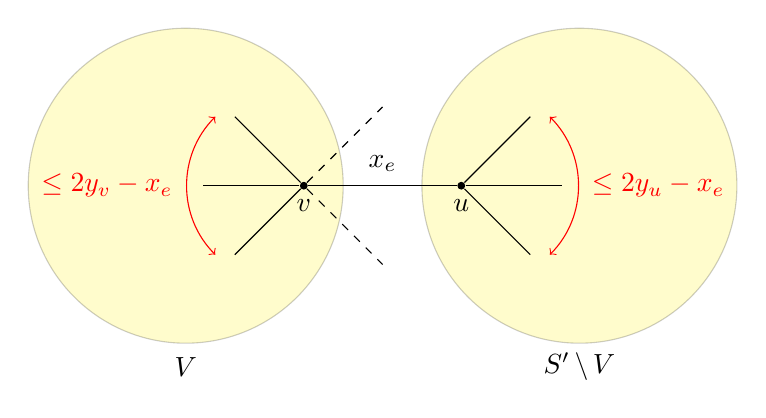
\begin{tikzpicture}
    	\draw [fill = yellow, opacity = 0.2] (-1.5, 0) circle [radius = 2];
    	\draw [fill = yellow, opacity = 0.2] (3.5, 0) circle [radius = 2];	
	\draw (0, 0) node[circle, inner sep=1pt, fill = black, label = {below:{$v$}}] (v) {}; 
        \draw (2, 0) node[circle, inner sep=1pt, fill = black, label = {below:{$u$}}] (u) {};     
        \node at (-1, 1) (a) {};
        \node at (-1.4, 0) (b) {};
        \node at (-1, -1) (c) {};
        \node at (3, 1) (d) {};
        \node at (3.4, 0) (e) {};
        \node at (3, -1) (f) {};
        \draw (u) to (v);
        \draw (v) to (a);
        \draw (v) to (b);
        \draw (v) to (c);
        \draw (u) to (d);
        \draw (u) to (e);
        \draw (u) to (f);
        \draw [dashed] (v) to (1, 1);
        \draw [dashed] (v) to (1, -1);
        \draw [<->, bend right = 45, color = red] (a) to (c);
        \draw [<->, bend left = 45, color = red] (d) to (f);
        \node [color = black, above = 0.05cm] at (1, 0) {$x_e$};
        \node [color = red] at (-2.5, 0) {$\leq 2y_v - x_e$};
        \node [color = red] at (4.5, 0) {$\leq 2y_u - x_e$};
        \node at (-1.5, -2.3) {$V$};
        \node at (3.5, -2.3) {$S' \, \backslash \, V$};
    \end{tikzpicture}
    \caption{Shrinking the edge $x_e$ between the nodes $u$ and $v$}
    \label{fig:shrink}    
\end{figure}
\item<2-> If $2y_u - x_e \leq x_e$, we can add $u$ to the $V$-side of the cut
\item<3-> Safe shrinking
\end{itemize}
\end{frame}

\begin{frame}{Shrinking Heuristic (Cont'd)}
\begin{itemize}
\item<1-> While there are more than two nodes in the graph, repeat the following:
\item<2-> For every edge, check if $\exists$ a safe shrinking
\item<3-> If $u$ and $v$ are to be merged:
	\begin{itemize}
	\item<4-> Make them into a \alert{super node}
	\item<5-> Merge incoming edges, combining weights
	\item<6-> Assign a new $y_{\{u, v \}}$ to the supper node: $y_u + y_v - x_{uv}$
	\item<7-> Update a value $m_{\{u, v \}}$, representing the maximum $y_k$ for any node $k$ in the super node
	\end{itemize}
\item<8-> After termination, either:
	\begin{itemize}
	\item<9-> We end up with exactly two nodes: \alert{represents the cut}, or
	\item<10-> We fail to find safe shrinking: run the flow algorithm on the \alert{smaller} network
	\end{itemize}
\end{itemize}
\end{frame}

\begin{frame}{Shrinking Heuristic - Experimental Results}

\begin{table}
\caption{Computational results for the heuristic GSEC separation} \label{tbl:results1}
\begin{minipage}{12cm}
\begin{center}
\resizebox{.55\textwidth}{!}{
\begin{tabular}{l l l l l l l l}
\hline \\
	&	\multicolumn{3}{l}{LP GSEC Sep.}	&	&	\multicolumn{3}{l}{Heuristic GSEC Sep.} \\
\cline{2-4}  \cline{6-8} \\
Instance	&	Obj.		&	Cuts		&	Time		&	&	Obj.		&	Cuts		&	Time		\\
\hline \\
ulysses22	&	-1964.93	&	16	&	1		&	&	-1964.93	&	13	&	<1	\\
bayg29		&	-44.35		&	33	&	4		&	&	-44.35		&	14	&	<1	\\
st70		&	-6433.23	&	94	&	423		&	&	-6433.23	&	26	&	1	\\
rd100		&	-10119.1	&	189	&	2501	&	&	-10119.1	&	35	&	2	\\
eil101		&	-8988.51	&	73	&	1108	&	&	-8988.51	&	17	&	5	\\
lin105		&				&	N/A	&	t.l.	&	&	-87.93		&	354	&	4371\\
gr137		&	-13070.5	&	112	&	4306	&	&	-13070.5	&	26	&	19	\\
pr152		&	984.54		&	13	&	10780	&	&	984.54		&	13	&	2	\\
gr202		&				&	N/A	&	t.l.	&	&	-19859.1	&	48	&	70	\\
ts225		&	1296.11		&	0	&	8466	&	&	1296.11		&	0	&	14	\\
gr431		&				&	N/A	&	t.l.	&	&	-41751		&	123	&	823	\\
p654		&				&	N/A	&	t.l.	&	&	-65478.8	&	71	&	1068\\
gr666		&				&	N/A	&	t.l.	&	&	-65273.1	&	169	&	54	\\
\hline
\end{tabular} }
\end{center}
\end{minipage}
\end{table}

\end{frame}

%%%%%%%%%%%%%%%%%%%%%%%%%%%%%%%%%%%%%%%%%%%%%%%%%%%%%%%%%%%%%%%%%%%%%%%%%%%%%%%%%%%%%%%%%%%%%%%%%%%%%%%%%%%%%%%%%%%%%%%%%%%%%%%
\section{Ordered Instances of the Scheduling Problem}

\begin{frame}{Introduction}
	\begin{itemize}
    	\item<1-> The resources are indivisible
        \item<2-> The system is deterministic (no stochastic scheduling)
        \item<3-> The objective is to allocate scarce resources to activities/customers/players so that a level of \alert{fairness} is guaranteed
    	\item<4-> We are interested in instances of the problem which can be approximated with any desired precision (PTAS)
		\begin{itemize}
        	\item<5-> \alert{Ordered instances}: precedence among resources
        \end{itemize}
    \end{itemize}

\end{frame}

\begin{frame}{Preliminaries}
	\begin{itemize}
    	\item<1-> We have a set of $m$ players $\cP = \{p_1, \, p_2, \, \ldots, \, p_m  \}$
        \item<2-> Who compete for a set of $n$ resources $\cI = \{x_1, \, x_2, \, \ldots, \, x_n \}$
        \item<3-> Each player has positive valuations for (is \emph{interested} in) only subsets of the resources
        \item<4-> Interests are given as input via a bipartite graph $H = (\cI, \, \cP, \, E)$
        \item<5-> A \alert{feasible} solution is an assignment of resources to players such that:
        \begin{itemize}
         	\item<6-> Each player only receives a set of items from her neighbourhood in $H$
            \item<7-> Each item is assigned to at most one player
        \end{itemize}
        \item<8-> The utility for each player is the sum of resource values assigned to her
    \end{itemize}
\end{frame}

\begin{frame}{Fairness I}
	\begin{itemize}
    	\item<1-> Two factors determine the type of the problem:
        	\begin{itemize}
            	\item<2-> The objective function
                \item<3-> The valuations for resources
            \end{itemize}
        \item<4-> Fairness is encoded in the objective function    
		\item<5-> Objective functions in this presentation:
        	\begin{itemize}
            	\item<6-> Maximize the minimum utility: \alert{Max-Min Fair Allocation} (\alert{Santa Claus})
                \item<7-> Minimize the maximum utility: \alert{Min-Max Fair Allocation} (\alert{$R \, | \, | \, C_{\max}$}) 
            \end{itemize}   
        \item<8-> The goal in the Max-Min problem: maximize the \emph{happiness} of the least happy player
        \item<9-> The goal in the Min-Max problem: minimize the \emph{load} of the most heavily-loaded player (makespan)
    \end{itemize}
\end{frame}
\begin{frame}
    \begin{itemize}
		\item<1-> Resource values in this presentation: 
        	\begin{itemize}
            	\item<2-> For Max-Min: resource $x_j$ has a \emph{value} $v_j$ to all who are interested in $x_j$ and $0$ to others
            	\item<3-> For Min-Max: resource $x_j$ has a \emph{cost} $v_j$ to all who are interested in $x_j$ and $\infty$ to others 
                \item<4-> Different resources may have different values
                \item<5-> This type of valuation is known as the \alert{restricted} version of the problem, \emph{e.g.}, \alert{restricted Santa Claus} or \alert{restricted $R \, | \, | \, C_{\max}$}
			\end{itemize}
    \end{itemize}
\end{frame}

\begin{frame}{Ordered Instances I}
	\begin{definition}[Adjacency Property]
    	Let $H = (X, \, Y, \, E)$ be a bipartite graph. An ordering $<_X$ of $X$ in $H$ has the \emph{adjacency property} if for each vertex $y \in Y$, the neighbourhood of $y$ in $X$ denoted by $N(y)$ consists of vertices that are consecutive in $<_X$.	
	\end{definition}
    A graph $H$ is said to be \alert{convex} if it has such an ordering on $X$
\end{frame}

\begin{frame}{Ordered Instances II}
    Or equivalently, 
    \begin{definition}[Min Ordering]
    	In the bipartite graph $H = (X, \, Y, \, E)$, an ordering $<_X$ satisfies the \emph{min ordering} property if the following holds: if $x <_X x'$ and $y <_X y'$ and $x \sim y'$ and $x' \sim y$, then \alert{$x \sim y$}
    	\begin{figure}
        		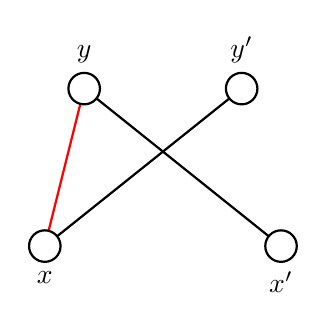
\begin{tikzpicture}
        			\draw[thick] (0, 0) -- (2.5, 2);
       				\draw[thick] (3, 0) -- (0.5, 2);  
        			\draw [red, thick] (0, 0) -- (0.5, 2);
					\draw [draw = black, fill = white, thick] (0, 0) circle (0.2cm);
   					\draw [draw = black, fill = white, thick] (3, 0) circle (0.2cm);
					\draw [draw = black, fill = white, thick] (0.5, 2) circle (0.2cm);
   					\draw [draw = black, fill = white, thick] (2.5, 2) circle (0.2cm);
    				\node[below = 0.2cm] at (0, 0) {$x$};
    				\node[below = 0.2cm] at (3, 0) {$x'$};
        			\node[above = 0.2cm] at (0.5, 2) {$y$};
        			\node[above = 0.2cm] at (2.5, 2) {$y'$};        
				\end{tikzpicture}
		\end{figure}
    \end{definition}
\end{frame}

\begin{frame}{Ordered Instances III}
	\begin{itemize}
    	\item<1-> Assume the neighbourhood of players forms an intervals in the set of resources
        \item<2-> Order the players lexicographically:
       	\begin{itemize}
        	\item<3-> First, based on the \alert{left boundary} of their neighbourhoods
            \item<4-> If they share the left boundary, based on the \alert{right boundary}
        \end{itemize}
        \item<5-> \alert{Problem:} Proper inclusions make it difficult to obtain a PTAS
    \end{itemize}
\end{frame}


\begin{frame}{Ordered Instances IV}
	\begin{definition}[Enclosure Property]
Let $H = (X, \, Y, \, E)$ be a bipartite graph. An ordering $<_X$ of $X$ in $H$ has the enclosure property if for each pair of vertices $y, y' \in Y$ for which $N(y) \subseteq N(y')$ in $X$, the vertices of $N(y') \, \backslash \, N(y)$ appear consecutively in $<_X$. We say that the graph $H$ as the enclosure property if such an ordering of the vertices of $H$ exists.	
	\end{definition}
    A graph $H$ is said to be \alert{proper convex} or \emph{inclusion-free convex} if it satisfies the enclosure property
\end{frame}

\begin{frame}{Ordered Instances V}
    Or equivalently, 
    \begin{definition}[Min-Max Ordering]
    	In the bipartite graph $H = (X, \, Y, \, E)$, an ordering $<_X$ satisfies the \emph{min-max ordering} property if the following holds: if $x <_X x'$ and $y <_X y'$ and $x \sim y'$ and $x' \sim y$, then \alert{$x \sim y$} \textbf{and} \alert{$x' \sim y'$}
    	\begin{figure}
        		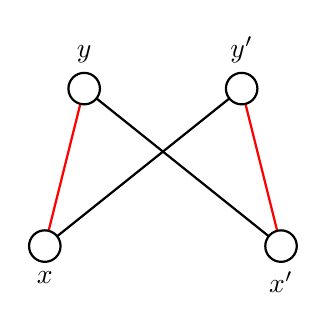
\begin{tikzpicture}
        			\draw[thick] (0, 0) -- (2.5, 2);
       				\draw[thick] (3, 0) -- (0.5, 2);  
        			\draw [red, thick] (0, 0) -- (0.5, 2);
			        \draw [red, thick] (3, 0) -- (2.5, 2);                    
					\draw [draw = black, fill = white, thick] (0, 0) circle (0.2cm);
   					\draw [draw = black, fill = white, thick] (3, 0) circle (0.2cm);
					\draw [draw = black, fill = white, thick] (0.5, 2) circle (0.2cm);
   					\draw [draw = black, fill = white, thick] (2.5, 2) circle (0.2cm);
    				\node[below = 0.2cm] at (0, 0) {$x$};
    				\node[below = 0.2cm] at (3, 0) {$x'$};
        			\node[above = 0.2cm] at (0.5, 2) {$y$};
        			\node[above = 0.2cm] at (2.5, 2) {$y'$};        
				\end{tikzpicture}
		\end{figure}
    \end{definition}
\end{frame}

%%%%%%%%%%%%%%%%%%%%%%%%%%%%%%%%%%%%%%%%%%%%%%%%%%%%%%%%%%%%%%%%
\subsection{Background}

\begin{frame}{Related Work I}
	Restricted Max-Min Fair Allocation (Santa Claus):
	\begin{itemize}
		\item<2-> Hardness results:
        \begin{itemize}
        	\item<3-> A $\frac{1}{2}$ inapproximability follows from the work of Lenstra, Shmoys, and Tardos \cite{LST90} 
		\end{itemize}
        \item<4-> Approximations:
        \begin{itemize}
            \item<5-> Asadpour et al. provided a $\frac{1}{4}$ \alert{estimation} algorithm via local search \cite{AFS08}
            \item<6-> The exponential running time of the local search in \cite{AFS08} was later improved to quasipolynomial ($n^{\mathcal{O}(\log n)}$) by Pol\'{a}\v{c}ek and Svensson \cite{PS12}
            \item<7-> Recently, Annamalai, Kalaitzis, and Svensson managed to give a \alert{$\frac{1}{13}$} approximation which runs in polynomial time \cite{AKS14}
        \end{itemize}
        \item<8-> PTAS:
        \begin{itemize}
            \item<9-> Alon et al. provided a PTAS for the case where the graph $H$ is a complete bipartite graph \cite{AAWY98}
            \item<10-> Jansen improved the running time of the PTAS by Alon et al. \cite{Jansen10}
            \item<11-> Muratore et al. \cite{MSW10} and Schwarz \cite{Schwarz10} provide PTASs on instances with \emph{nested} and \emph{tree-precedence} intervals respectively.
        \end{itemize}
	\end{itemize}
\end{frame}

\begin{frame}{Related Work II}
	Restricted Min-Max Fair Allocation ($R \, | \, | \, C_{\max}$):
    \begin{itemize}
    	\item<2-> Hardness results:
        \begin{itemize}
        	\item<3-> A famous $\frac{3}{2}$ inapproximability by Lenstra, Shmoys, and Tardos \cite{LST90}
        \end{itemize}
        \item<4-> Approximations:
        \begin{itemize}
        	\item<5-> Lenstra, Shmoys, and Tardos also provided a $2$-approximation using the \alert{Assignment LP} formulation.
            \item<6-> Svensson provided a \alert{$\frac{33}{17} + \varepsilon$ estimation} algorithm for small values of $\varepsilon$ \cite{Svensson11}
            \item<7-> Ebenlender, Krc\'{a}l, and Sgall \cite{EKS08} provided a \alert{$1.75$} approximation algorithm for the special case where each resource (job) can be assigned to at most two players (machines)
        \end{itemize}
        \item<8-> PTAS:
        \begin{itemize}
            \item The results of Alon et al. \cite{AAWY98}, Jansen \cite{Jansen10}, Muratore et al. \cite{MSW10}, and Schwarz \cite{Schwarz10} hold for the $R \, | \, | \, C_{\max}$ as well.
        \end{itemize}
    \end{itemize}
\end{frame}

%%%%%%%%%%%%%%%%%%%%%%%%%%%%%%%%%%%%%%%%%%%%%%%%%%%%%%%%%%%%%%%%
\subsection{Our Contribution}
\begin{frame}{Our Contribution}	
    \begin{itemize}
    	\item<1-> In this thesis, we provide:
        \begin{itemize}
	    	\item<2-> A PTAS for the restricted Santa Claus problem on inclusion-free convex graphs
        	\item<3-> A conceptually dual PTAS for the problem of $R \, | \, | \, C_{\max}$ on inclusion-free convex graphs
        	\item<4-> A PTAS the tree-precedence intervals (\alert{laminar families}) and extensions of the laminar families.
    	\end{itemize}
		\item<4-> The work presented in:
    	\begin{itemize}
    		\item<5-> K. K., R. Krishnamurti, A. Rafiey, G. Stamoulis:
\alert{PTAS for Ordered Instances of Resource Allocation Problems}, \emph{FSTTCS 2013} \cite{KKRS13}.
        	\item<6-> K. K., R. Krishnamurti, A. Rafiey, G. Stamoulis:
\alert{PTAS for Ordered Instances of Resource Allocation Problems with Restrictions on Inclusions} \emph{(submitted paper)} \cite{KKRS16}.
		\end{itemize}
    \end{itemize}
\end{frame}

\begin{frame}{Our Method: Santa Clause Prbolem I}
	\begin{itemize}
    	\item<1-> Turn the problem into a feasibility test: does there exist an allocation in which each player receives a utility of at least $t$ for a \alert{guessed} value of $t$?
        \item<2-> A generalization of \alert{Hall's condition} and first prove its necessity for existence of a ``$t$-assignment''
        \item<3-> Constructively prove its sufficiency for a \alert{$(1 - \frac{4}{k + 1})$} approximation
    \end{itemize}
\end{frame}

\begin{frame}{Our Method: Santa Claus Problem II}
	\begin{itemize}
    	\item<1-> For a given $k$, round \alert{up} resource values which are greater than $\frac{1}{k}$ geometrically:
    	\begin{itemize}
    	    \item<2-> $\Big( \frac{1}{k}(1 + \frac{1}{k})^i, \, \frac{1}{k}(1 + \frac{1}{k})^{(i + 1)} \Big]  \rightarrow \frac{1}{k}(1 + \frac{1}{k})^{(i + 1)}$.
    	\end{itemize}
	\end{itemize}
	\begin{lemma}[The Alignment Lemma]<2->
    	For any given assignment of items to players, the items can be \alert{aligned} to the right of the neighbourhood of each player (going from right to left in the lexicographical order) in such a way that the total loss of approximation quality is at most $\frac{1}{k}$
    \end{lemma}
    \begin{lemma}[The Retrieval Lemma]<3->
    	Any right-aligned assignment that does not leave any item \alert{stranded} can be recreated for all players, from right to left, only from a \alert{signature vector} with loss of approximation quality no more than $\frac{2}{k}$
    \end{lemma}
\end{frame}

\begin{frame}{Our Method:Santa Claus Problem III}
	\begin{itemize}
    	\item<1-> Run a dynamic programming algorithm
        \item<2-> Due to the rounding, only polynomially many signature vectors (\alert{input vectors)}
        \item<3-> Going form right to left for players, (try to) assign items to players in a right-aligned fashion for each input vector
        \item<4-> Keep track of \alert{successful} input vectors
        \item<5-> The running time: $\bigO{(m + n)nm^{2(C+1)}}$, in which $C \leq k^{1.4}$
        \item<6-> Approximation factor: $1 - \frac{3}{k}$ form the \alert{two lemmas} times $\frac{1}{1 + \frac{1}{k}}$ form the \alert{rounding}
	\end{itemize}
\end{frame}

\begin{frame}{Our Method: $R \, | \, | \, C_{\max}$}
    \begin{itemize}
        \item<1-> Change of notation:
            \begin{itemize}
                \item<2-> Players $\rightarrow$ Machines, $M = \{M_1, \, M_2, \, \ldots, \, M_m\}$
                \item<3-> Resources $\rightarrow$ Jobs, $J = \{J_1, \, J_2, \, \ldots, \, J_n\}$
                \item<4-> Values $\rightarrow$ Processing times, $p_1, \, p_2, \, \ldots, \, p_n$
            \end{itemize}
        \item<5-> Turn the problem into a feasibility test: does there exist an assignment of \alert{all} jobs in which each machine has a makespan of at most $t$ for a \alert{guessed} value of $t$?
        \item<6-> Using similar ideas (and a slightly different rounding scheme), we constructively provide a $1 + \frac{4}{k} + \frac{3}{k^2}$ approximation
    	\item<7-> For a given $k$, round \alert{down} job processing times which are greater than $\frac{1}{k}$ geometrically:
    	\begin{itemize}
    	    \item<8-> $\Big[ \frac{1}{k}(1 + \frac{1}{k})^i, \, \frac{1}{k}(1 + \frac{1}{k})^{(i + 1)} \Big)  \rightarrow \frac{1}{k}(1 + \frac{1}{k})^i$.
    	\end{itemize} 
    	\item<9-> The running time: $\bigO{(m + n)mn^{2(C + 1)}}$, in which $C \leq 1.4$
    \end{itemize}
\end{frame}

\begin{frame}{Our Method: Laminar Families of Sets I}
	\begin{itemize}
		\item<1-> So far, we have restricted inclusions by disallowing proper inclusions. 
        \item<2-> Another set of ordered instances: neighbourhoods of machines $M_1, \, M_2, \, \ldots, \, M_m$ form \alert{Laminar} families in the set of jobs $J$.
	\end{itemize}
    \begin{definition}[Laminar Families]<3->
    	Assume $H$ is a collection of subsets of a ground set $X$ (i.e., a \alert{hypergraph}). $H$ is a \emph{laminar family} (or a \alert{hierarchical system}) if for every two elements $e_1, \, e_2 \in H$, either
        \begin{itemize}
        	\item $e_1 \, \cap \, e_2 = \varnothing$, or
            \item $e_1 \subseteq e_2$, or
            \item $e_2 \subseteq e_1$
        \end{itemize}
    \end{definition}
\end{frame}

\begin{frame}{Our Method: Laminar Families of Sets II}
    \begin{itemize}
        \item<1-> Laminar families represent hierarchical relations between sets
        \item<2-> Every machine can process all the jobs in its subtree
    \end{itemize}
    \begin{figure}
        \begin{center}
            \includegraphics[width=6cm]{laminar.eps}
        \end{center}
    \end{figure}
\end{frame}

\begin{frame}{Our Method: Laminar Families of Sets III}
    \begin{itemize}
        \item<1-> Assume the tree structure is given
        \item<2-> We start the assignment from the leaves of the tree:
        \begin{itemize}
            \item<3-> Identify the \alert{successful} assignment for the leaves
            \item<4-> In polynomial time, merge the successful assignment vectors for parents of the leaves and get their \emph{input vectors}
            \item<5-> Remove the leaves and continue the process        
        \end{itemize}
        \item<6-> The procedures results in a $1 + \frac{2}{k} + \frac{1}{k^2}$ approximation
        \item<7-> The running time: $\bigO{m(n+1)n^{2(C + 1)}}$, in which $C \leq k ^ {1.4}$
    \end{itemize}
\end{frame}

\begin{frame}{Our Method: Extended Laminar Families of Sets}
\end{frame}

\begin{frame}{Future Directions}
	\begin{itemize}
    	\item<1-> Convex graphs in general
        \item<2-> Items on the trees (partial orders on resources)
        \item<3-> Finding other graph classes that admit a PTAS
        	\begin{itemize}
            	\item<4-> Trivially perfect bigraphs
                \item<5-> Chordal bigraphs
                \item<6-> $\ldots$
            \end{itemize}
    \end{itemize}
\end{frame}
%%%%%%%%%%%%%%%%%%%%%%%%%%%%%%%%%%%%%%%%%%%%%%%%%%%%%%%%%%%%%%%%%%%%%%%%%%%%%%%%%%%%%%%%%%%%%%%%%%%%%%%%%%%%




%%%%%%%%%%%%%%%%%%%%%%%%%%%%%%%%%%%%%%%%%%%%%%%%%%%%%%%%%%%%%%%%%%%%%%%%%%%%%%%%%%%%%%%%%%%%%%%%%%%%%%%%%%%%%%%%%%%%%%%%%%%%%%%
\section{Conclusion and Future Work}

\begin{frame}{Summary}
\begin{itemize}
\item<1-> We analyzed a shrinking heuristic for separation of GSECs
	\begin{itemize}
	\item<2-> \alert{Significant improvement} in the running time compared to LP separation
	\end{itemize}
\item<3-> We studied the benefits of using odd component heuristic for separation of Primitive Combs
	\begin{itemize}
	\item<4-> In most cases: \alert{improves} the solution quality, spending a reasonable amount of extra time
	\item<5-> In others: generates extra cuts in the added time while the solution quality does not improve (\alert{optimality certificate})
	\item<6-> In some cases: achieves \alert{nothing} while spending a long time
	\item<7-> Trade-off?
	\end{itemize}
\end{itemize}
\end{frame}

\begin{frame}{Future Work}
\begin{itemize}
\item<1-> Heuristics for many other families of cuts (valid inequalities)
	\begin{itemize}
	\item<2-> e.g., General Comb Inequalities, Cycle-Cover, $\ldots$
	\end{itemize}
\item<3-> Analyze the interplay between the cuts and the order they are introduced in
\end{itemize}
\end{frame}

\plain{Thank You!}

\begin{frame}{Publication}
\begin{itemize}
    \item Published papers:
    \begin{itemize}
        \item[\cite{KKRS13}]
        \item[\cite{KK16}]
    \end{itemize}
    \item Submitted papers:
    \begin{itemize}
        \item[cite{}]
    \end{itemize}
        
\end{itemize}

\end{frame}

\begin{frame}[allowframebreaks]{References}

	\bibliography{references}
    \bibliographystyle{abbrv}

\end{frame}

\end{document}
